\chapter{Results}
\label{ch:results}

This chapter will outline results of experiments conducted for this thesis,
according to the methodology outlined in the previous chapter.
Firstly, Chapter~\ref{sec:dda} delivers explorative analysis of all three
collected data sets, comparing them along several dimensions.
Afterwards, the developed models will be introduced along with an evaluation
of their predictive performance.
Included features, model architectures, necessary preprocessing steps and results will
be described for linear baseline (ch.~\ref{sec:linear_models}),
deep feedforward (ch.~\ref{sec:deep1}) and more complex deep models
(ch.~\ref{sec:deep_combined}).

\subsection{Descriptive Data Analysis}
\label{sec:dda}

Developing machine learning models for predicting certain outcomes requires
an understanding of the underlying data.
Insights derived from descriptive data analysis are useful in all steps of the
modeling process, e.g., for preprocessing, feature extraction and evaluation
of model performance.
For this thesis, exploratory data analysis also serves the purpose of establishing
differences between the three examined data sets.
The upcoming sections compare the collected data sets along the dimensions of
engagement metrics (ch.~\ref{sec:engagement_stats}), network characteristics
(ch.~\ref{sec:network_stats}) and general account activity (ch.~\ref{sec:activity_stats}).
Prior to presenting the results of this analysis, a few remarks about presentation
have to be made.
In almost all cases, data is discretized to improve clarity.
Here, all created bins, e.g., in histograms, are left-inclusive and right-exclusive.
For example, the bin `1-10k' denotes all observations between 1,000 and
9,999 (for a variable scaled as an integer).
In addition, all represented distributions are normalized to account for varying
data set sizes and improve comparability.

\subsubsection{Engagement statistics}
\label{sec:engagement_stats}

Examining engagement statistics for all three data sets is crucial since the goal
of this thesis is to predict these variables.
This section will therefore compare retweet and favorite distribution for 
celebrity, politician and corporate tweets.

\begin{table}
\centering
\begin{tabular}{lrrr}
\toprule
Retweets & Celebrities & Politicians & Companies \\
\midrule
Mean & 1,629.8 & 318.4 & 15.1 \\
Median & 176.0 & 23.0 & 1.0 \\
\midrule
Favorites & Celebrities & Politicians & Companies \\
\midrule
Mean & 6,135.6 & 832.9 & 40.3 \\
Median & 1117.0 & 69.0 & 1.0 \\
\midrule
Pearson correlation & Celebrities & Politicians & Companies \\
\midrule
Correlation coefficient & 0.9188 & 0.9457 & 0.9803 \\
\bottomrule
\end{tabular}
\caption{Summary of engagement statistics}
\label{tab:engagement_summary}
\end{table}

Table~\ref{tab:engagement_summary} indicates that celebrity tweets are engaged
with most often.
This holds true when looking at central tendency statistics (mean and median)
for retweet and favorite counts.
Moreover, in this sample politician tweets are more popular compared to tweets from corporate
accounts.
For all three data sets, strong correlation between the number of favorites and retweets can
be stated.
This observation is useful for later model development, because it can be concluded that
both variables should be predictable using similar statistical models, e.g.,
a multi-output model with differently scaled weights in the last layer.
The differences between mean and median values point to skewness in the
underlying distributions.
Since the calculated means are significantly larger than their respective
median values, observations should extend farther to the right
of the distributions.
This finding can be explained twofold. 
Firstly, retweet and favorite counts have an obvious  minimum of zero.
Secondly, a small number of very popular tweets constitute outliers which largely
influence the mean calculation.
In order to examine engagement distributions in more detail, Fig.~\ref{fig:retw_distr} and
Fig.~\ref{fig:fav_distr} illustrate engagement statistics which are discretized into logarithmic bins (base 10).
Above discretization also corresponds to the classes used for the classification models
of this thesis.

\begin{figure}[h]
\centering
\begin{subfigure}{.33\textwidth}
  \centering
  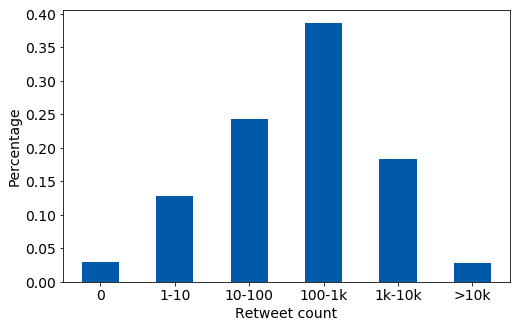
\includegraphics[width=.95\linewidth]{img/celeb_retw_distr}
  \caption{Celebrity data set}
  \label{fig:retw_distr_sub1}
\end{subfigure}%
\begin{subfigure}{.33\textwidth}
  \centering
  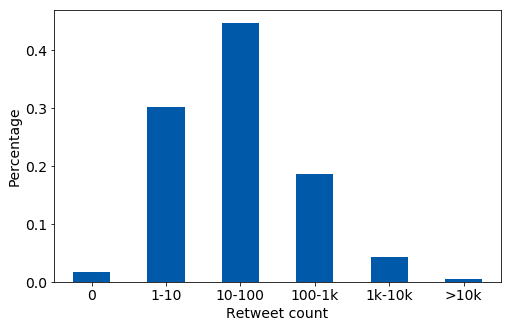
\includegraphics[width=.95\linewidth]{img/polit_retw_distr}
  \caption{Politician data set}
  \label{fig:retw_distr_sub2}
\end{subfigure}
\begin{subfigure}{.33\textwidth}
  \centering
  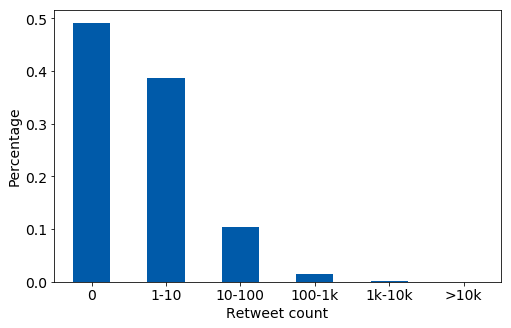
\includegraphics[width=.95\linewidth]{img/corp_retw_distr}
  \caption{Company data set}
  \label{fig:retw_distr_sub3}
\end{subfigure}%
\caption{Retweet distributions}
\label{fig:retw_distr}
\end{figure}

\begin{figure}[h]
\centering
\begin{subfigure}{.33\textwidth}
  \centering
  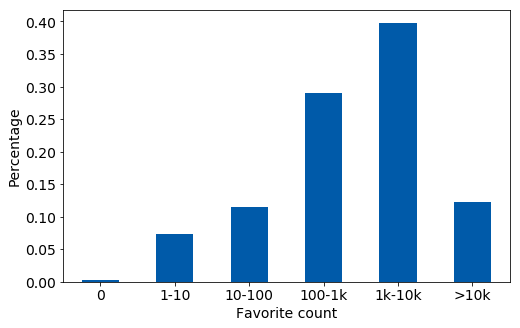
\includegraphics[width=.95\linewidth]{img/celeb_fav_distr}
  \caption{Celebrity data set}
  \label{fig:fav_distr_sub1}
\end{subfigure}%
\begin{subfigure}{.33\textwidth}
  \centering
  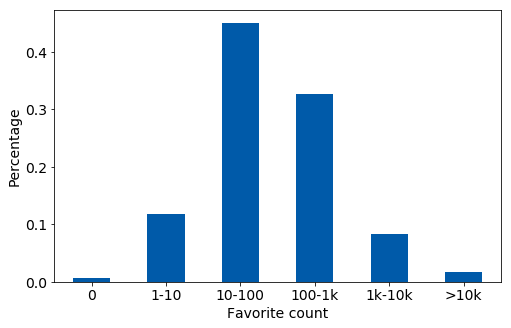
\includegraphics[width=.95\linewidth]{img/polit_fav_distr}
  \caption{Politician data set}
  \label{fig:fav_distr_sub2}
\end{subfigure}
\begin{subfigure}{.33\textwidth}
  \centering
  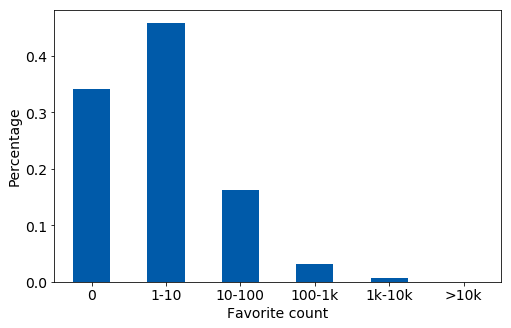
\includegraphics[width=.95\linewidth]{img/corp_fav_distr}
  \caption{Company data set}
  \label{fig:fav_distr_sub3}
\end{subfigure}%
\caption{Favorite distributions}
\label{fig:fav_distr}
\end{figure}

All three data sets possess class imbalance, i.e., some classes are more likely
to occur than others.
Here, differences in class probabilities are significant across data sets
and variables, with the most common class
containing close to or more than 40\% of all observations and some classes
hardly being represented at all.
Looking at retweets it can be stated that celebrity and politician distributions
have a Gaussian-like shape, where the central tendency of celebrity tweets is
farther to the right.
Company retweet classes seem to be more exponentially shaped.
Moving to favorites, central tendencies of all distributions are clearly pushed to the right of the
spectrum, which accounts for the generally observed difference between favorite
and retweet counts.

The upcoming subsections further describe characteristics of the collected
data sets and provide possible explanations of the found discrepancies in
retweet and favorite distributions.

\subsubsection{Network statistics}
\label{sec:network_stats}

Prior work in this area suggests the importance of user data when predicting
popularity of created tweets.
The most obvious features in this category are the number of incoming and outgoing
connections, i.e., follower and friend counts in the context of Twitter.
This section shows the distribution of these variables in the previously
defined user groups and examines the correlation with engagement metrics.

\begin{table}
\centering
\begin{tabular}{lrrr}
\toprule
Number of followers & Celebrities & Politicians & Companies \\
\midrule
Mean & 10,255,423 & 331,944 & 357,023 \\
Median & 3,228,642 & 89,072 & 23,204 \\
Correlation w/ retweets & 0.1457 & 0.2828 & 0.0326 \\
Correlation w/ favorites & 0.1922 & 0.3423 & 0.0442 \\
\midrule
Number of friends & Celebrities & Politicians & Companies \\
\midrule
Mean & 5,587 & 3,775 & 5,513 \\
Median & 241 & 599 & 800 \\
Correlation w/ retweets & 0.1799 & 0.0030 & -0.0036 \\
Correlation w/ favorites & 0.1754 & 0.0092 & -0.0049 \\
\bottomrule
\end{tabular}
\caption{Summary of network statistics}
\label{tab:network_summary}
\end{table}

\begin{figure}[h]
\centering
\begin{subfigure}{.33\textwidth}
  \centering
  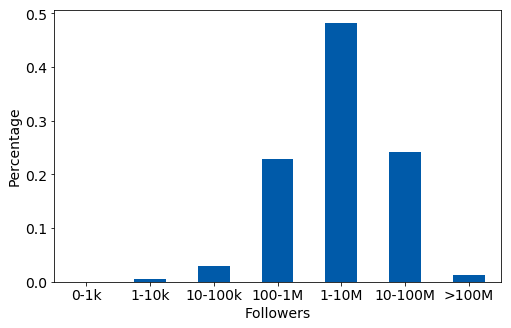
\includegraphics[width=.95\linewidth]{img/celeb_follow_distr}
  \caption{Celebrity data set}
  \label{fig:follow_distr_sub1}
\end{subfigure}%
\begin{subfigure}{.33\textwidth}
  \centering
  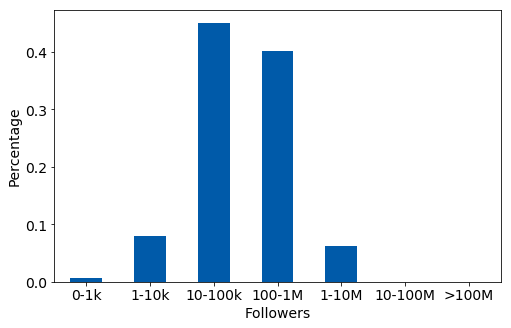
\includegraphics[width=.95\linewidth]{img/polit_follow_distr}
  \caption{Politician data set}
  \label{fig:follow_distr_sub2}
\end{subfigure}
\begin{subfigure}{.33\textwidth}
  \centering
  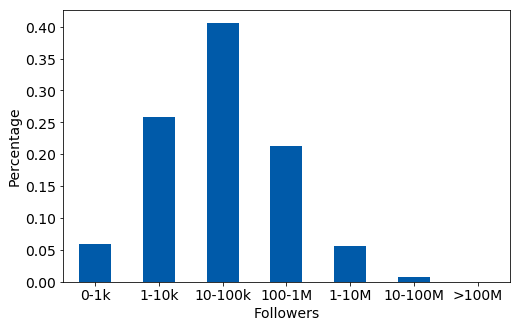
\includegraphics[width=.95\linewidth]{img/corp_follow_distr}
  \caption{Company data set}
  \label{fig:follow_distr_sub3}
\end{subfigure}%
\caption{Follower distributions}
\label{fig:follow_distr}
\end{figure}

Table~\ref{tab:network_summary} summarizes network statistics for all three
user groups.
It can be stated that celebrities tend to have the largest following on average,
followed by companies and politicians.
Most celebrities are followed by more than a million accounts, whereas the
majority of politicans and companies have followings smaller than 100 thousand
accounts (see Fig.~\ref{fig:follow_distr}).
Again, follower and friend distributions are skewed to the right across all
groups.
Considering the previously demonstrated differences in retweet and favorite
distributions, one could assume a correlation between number of followers
and tweet popularity.
However, linear correlation with retweet and favorites counts is nonexistent
(celebrities and companies) or only weakly positive (politicians).
Correlation coefficients are even lower for the number of friends a user
possesses.
The friend distributions have a similar shape, more than half of all users
follow less than 1,000 accounts (see Fig.~\ref{fig:friend_distr}).
The median value is highest for corporate accounts which seems logical, since
these accounts are probably most often managed using more manpower.
Particularly strong linear relationships between number of friends and engagement statistics can not
be found.

\begin{figure}[h]
\centering
\begin{subfigure}{.33\textwidth}
  \centering
  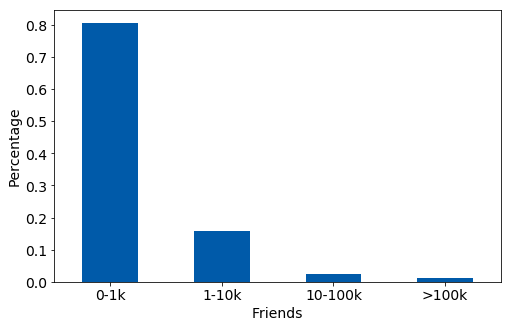
\includegraphics[width=.95\linewidth]{img/celeb_friend_distr}
  \caption{Celebrity data set}
  \label{fig:friend_distr_sub1}
\end{subfigure}%
\begin{subfigure}{.33\textwidth}
  \centering
  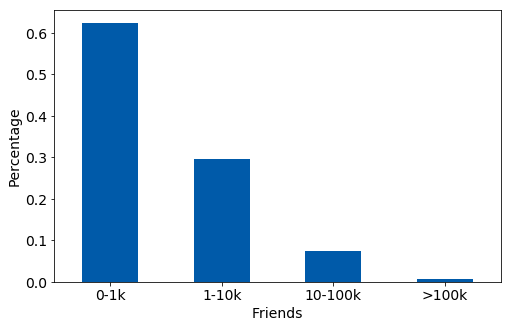
\includegraphics[width=.95\linewidth]{img/polit_friend_distr}
  \caption{Politician data set}
  \label{fig:friend_distr_sub2}
\end{subfigure}
\begin{subfigure}{.33\textwidth}
  \centering
  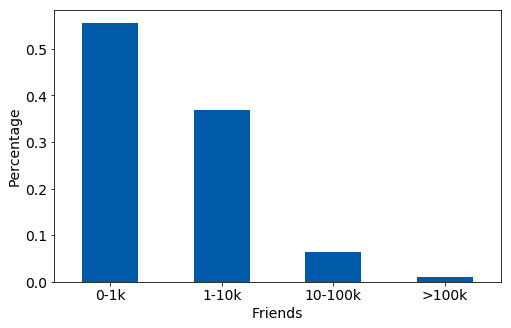
\includegraphics[width=.95\linewidth]{img/corp_friend_distr}
  \caption{Company data set}
  \label{fig:friend_distr_sub3}
\end{subfigure}%
\caption{Friend distributions}
\label{fig:friend_distr}
\end{figure}

\subsubsection{Activity statistics}
\label{sec:activity_stats}

Like network data, activity statistics have been used as features in previously
developed models which serve the purpose of retweet prediction.
Both feature groups can be classified in the category of contextual features,
as opposed to content features.
This section will describe account age and tweet frequency as indicators
for user activity.

\begin{figure}[h]
\centering
\begin{subfigure}{.33\textwidth}
  \centering
  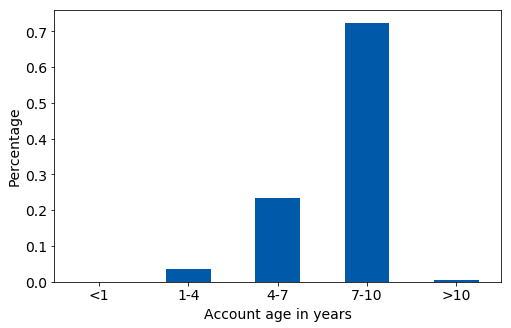
\includegraphics[width=.95\linewidth]{img/celeb_age_distr}
  \caption{Celebrity data set}
  \label{fig:age_distr_sub1}
\end{subfigure}%
\begin{subfigure}{.33\textwidth}
  \centering
  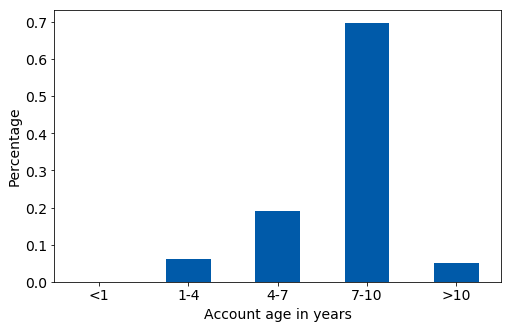
\includegraphics[width=.95\linewidth]{img/polit_age_distr}
  \caption{Politician data set}
  \label{fig:age_distr_sub2}
\end{subfigure}
\begin{subfigure}{.33\textwidth}
  \centering
  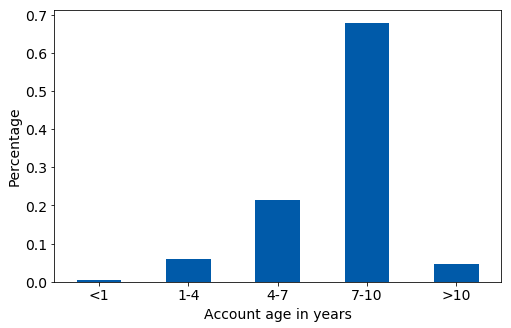
\includegraphics[width=.95\linewidth]{img/corp_age_distr}
  \caption{Company data set}
  \label{fig:age_distr_sub3}
\end{subfigure}%
\caption{Account age distributions}
\label{fig:age_distr}
\end{figure}

Fig.~\ref{fig:age_distr} shows the account age distributions, calculated for
each user group individually.
Superficially, the distributions look similar.
For all groups, around 70\% of all accounts are seven to ten years old, thus being
created two to four years after Twitter was opened for public access.
Earlier adopters mainly stems from the politician and company user groups, about
5\% of accounts in these groups are older than ten years.
There is hardly any skewness in the account age distribution, i.e., median and
mean values are close to each other.

\begin{figure}[h]
\centering
\begin{subfigure}{.33\textwidth}
  \centering
  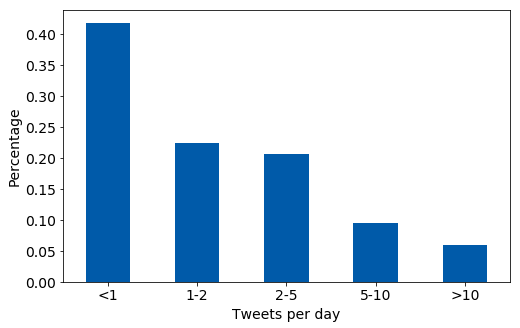
\includegraphics[width=.95\linewidth]{img/celeb_freq_distr}
  \caption{Celebrity data set}
  \label{fig:freq_distr_sub1}
\end{subfigure}%
\begin{subfigure}{.33\textwidth}
  \centering
  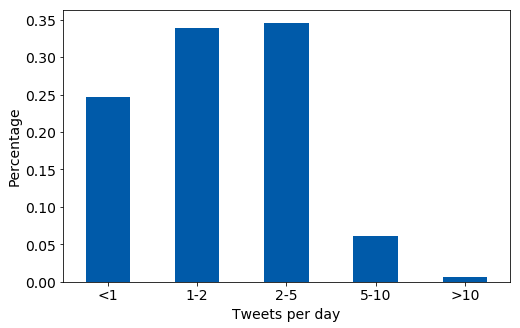
\includegraphics[width=.95\linewidth]{img/polit_freq_distr}
  \caption{Politician data set}
  \label{fig:freq_distr_sub2}
\end{subfigure}
\begin{subfigure}{.33\textwidth}
  \centering
  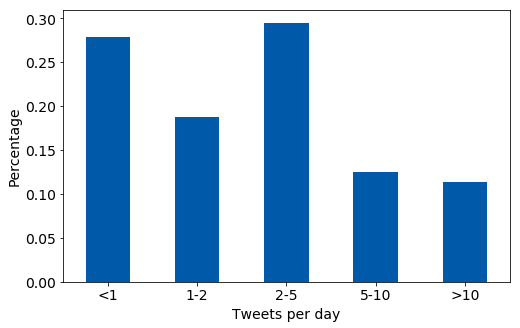
\includegraphics[width=.95\linewidth]{img/corp_freq_distr}
  \caption{Company data set}
  \label{fig:freq_distr_sub3}
\end{subfigure}%
\caption{Tweet frequency distributions}
\label{fig:freq_distr}
\end{figure}

Although accounts exemplify rougly the same age distribution across all user
groups, their activity level differ considerably (see Fig.~\ref{fig:freq_distr}).
Many celebrities do not average one tweet per day and the median for this group (1.20)
is lower than the respective counterparts for politicians and companies (1.75 resp. 2.16).
However, these numbers are not surprising, since many companies user their accounts
for daily customer support.
This could also explain the high percentage of accounts with more than ten tweets
per day in this group (so-called \textit{power users}).
It can also be stated that users from the politician user group tend to concentrate
in the range of under five tweets per day.
The 75th percentile is the lowest for all three user groups (2.83 tweets per day).
Neither account age nor tweet frequency show any direct linear correlation with
retweet or favorite counts for the collected tweets.
In more detail, all correlation coefficients are located between -0.1 and 0.1 (all
calculated values can be found in the appendix of this thesis).

This section concludes the descriptive data analysis part of this thesis.
Observations derived from these analyses are used in subsequent sections,
particularly for feature extraction and performance evaluation.


\section{Linear Models}
\label{sec:linear_models}

This section comprises results of linear engagement prediction models that
were trained as a baseline for later comparison with deep neural networks.
This kind of model evolution allows analysis of performance improvements
with regard to standardized metrics.
As is the case for all models, both multi-class classification and regression
models were developed for all three data sets.
This section starts with describing the model architecture (ch.~\ref{sub:lin_architecture}) and continues by detailling the training process (ch.~\ref{sub:lin_training}).
It concludes by summarizing results and analyzing model performance in more detail
(ch.~\ref{sub:lin_performance}).

\subsection{Model architecture}
\label{sub:lin_architecture}

\begin{figure}[h]
  \centering
  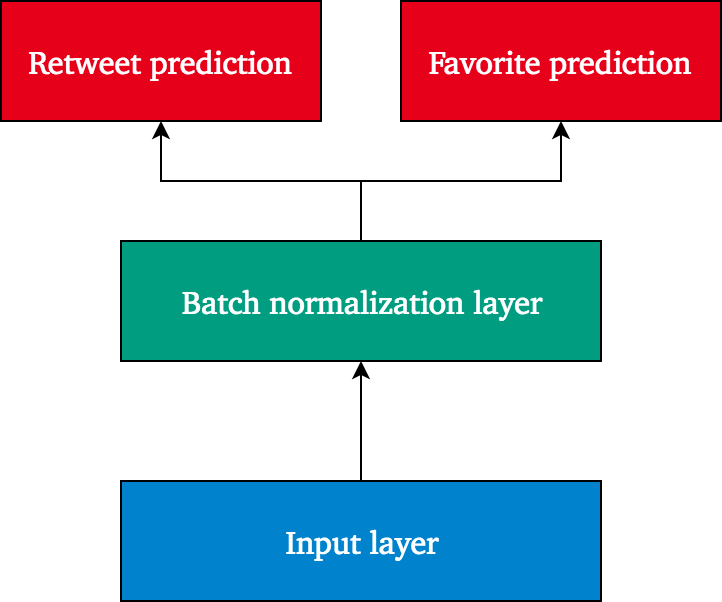
\includegraphics[height=8cm]{img/linear_model_architecture}
  \caption{General architecture of linear models}
\label{fig:linear_model_architecture}
\end{figure}

Fig.~\ref{fig:linear_model_architecture} illustrates the general architecture
of linear models trained in this work.
Firstly, inputs are normalized using a \textit{batch normalization} (see ch.~\ref{sub:dl_regularization})
layer in order to account for different scaling in the features.
As stated before, this layer type allows the model to undo normalization at
training time if it serves the purpose of better output representation.
The normalized inputs are then directly mapped onto two distinct outputs,
one for the number of retweets and one for the number of favorites.
In this case, regression and classification models only differ in their
respective type of prediction.
The regression model simply outputs two numbers representing retweet and
favorite estimates.
Hence, this constitutes a \textit{linear regression model}, because the output is not transformed.
Contrary, the classification model should output class probabilities for each
of the six predefined classes (see Table~\ref{tab:classification_buckets}).
As a result, the outputs have to be split according to the number of classes and transformed
using the \textit{sigmoid function} (see ch.~\ref{sub:dl_forward}).
This kind of model is called \textit{logistic regression} and is considered
a linear classifier despite the outputs being transformed using a non-linear
function.
The reason for that is the sole reliance on a linear combination of the
(normalized) inputs.

\begin{table}
\centering
\begin{tabular}{ll}
\toprule
Feature & Description \\
\midrule
URL count & Number of URLs \\
Hashtag count & Number of hashtags \\
Mention count & Number of mentioned users \\
Tweet length & Length in characters \\
Quoted tweet & Is tweet a quote? \\
\midrule
Follower count & Number of followers the tweet author has \\
Friend count & Number of friends the tweet author has \\
Verified status & Is the tweet author verified? \\
User listings & Number of lists tweet author was added to \\
User tweet count & Total number of tweets by tweet author \\
User overall tweet frequency & Tweets per day by tweet author \\
User favorite count & Total number of given favorites by tweet author \\
User overall favorite frequency & Number of given favorites per day by tweet author \\
User account age & Number of days since account creation \\
Hour of tweet creation & Hour of the day the tweet was created \\
\bottomrule
\end{tabular}
\caption{Linear model features}
\label{tab:structured_features}
\end{table}

All input features (see Table~\ref{tab:structured_features}) are directly derived
from collected tweet objects.
Since these objects contain information about the tweet author, no further data lookups
are necessary.
Consequently, these features can be extracted with minimal preprocessing, which
enables model application in a real-time prediction setting.
The structured inputs are separated into content (top half) and contextual
features (bottom half).
Activity statistics, i.e. frequencies, are calculated on a per-day basis,
the hour of tweet creation is given in \textit{Coordinated Universal Time (UTC)}.
The previouly described need for normalization becomes obvious, e.g., when
comparing scales for URL counts (usually 0-3) and account age (thousands of days).
Content features mainly incorporate information on the use of conversational
tools (URLs, mentions, hashtags), but do not model the tweet content itself.
In addition, contextual features comprise popularity and activity information
about the tweet author.

\begin{table}
\centering
  \begin{tabular}{lr}
    \toprule
    Class & Range \\
    \midrule
    1 & 0 \\
    2 & 1-9 \\
    3 & 10-99 \\
    4 & 100-999 \\
    5 & 1,000-9,999 \\
    6 & >10,000 \\
    \bottomrule
  \end{tabular}
  \caption{Classes for classification models}
  \label{tab:classification_buckets}
\end{table}

General model output types were previously described.
In short, regression models output a positive real-valued estimate of the
eventual favorite and retweet count.
Classification models on the other hand aim to predict the probability that
these counts are within a certain range.
The prefined ranges represent the output classes and are shown in Table~\ref{tab:classification_buckets}.
Basically, the classes represent a logarithmic scale of eventual engagement counts.
Since retweet and favorite counts are wide-ranging in all three data sets,
scaling the outputs logarithmically creates a more balanced class distribution.
As described in section~\ref{sec:engagement_stats} the underlying class distributions
are still far from uniform.
However, the data sets proved to be large enough to learn this slightly 
imbalaced distribution with more complex models (see subsequent sections).
Other common methods for handling class imbalance, e.g., penalizing misclassifications
in rare classes via class weights, did not improve results significantly.
Retweet and favorite prediction are treated equally, i.e., the final loss
is calculated by building the mean of loss values for the singular tasks.

After establishing model architecture including input and output types, the next
session will explain details about the training process.

\subsection{Training process}
\label{sub:lin_training}

Accurate model comparisons require a standardized setting regarding training
processes.
Therefore, the following paragraphs will describe important aspects of model training
used in this work.
In particular, data usage, training duration and choices of optimization
algorithm and cost functions will be explained and motivated.

Prior to training, all three data sets were split into training and validation
data according to a 90\%/10\% split.
Since the splitting process was undertaken after permutating the example order
randomly, class distributions in training and validation sets should be very
similar.
Training examples were used to learn the weights of the model, whereas validation
examples are not known to the algorithm during training.
Consequently, the unseen data could be used to derive an estimate of the model
generalizability.
Models were trained for a fix number of iterations, each iteration consisting
of a full pass over all training examples.
Here, training data was split into batches of 128 examples whose gradients
were averaged in order to derive weight updates.
Testing was conducted to determine the required number of iterations for
convergence in loss function minimization.
The regression models turned out to converge slower, so that these models
had to be trained for a longer period of time.
In summary, regression models were trained for 150 iterations, whereas classification
models already converged after 50 iterations.

After comparing multiple optimization algorithms on data samples, \textit{adaptive
moment estimation (Adam)} was used for all experiments in this work.
Recapping from ch.~\ref{sub:dl_optimization_algos}, this recently developed
algorithm adapts learning rates for each parameter based on mean and variance of
recent updates.
It therefore combines strengths of previously developed techniques such as
\textit{momentum} and \textit{RMSprop}.
Tests showed faster convergence and more stability of the training process, i.e.,
fewer iterations were needed to derive an acceptable minimum of the loss function.
The default parameters detailed in the background chapter turned out to be sufficient
for linear models and did not require adjustments.

\textit{Adam} was applied to the minimization of two different cost functions for
classification and regression models.
Mathematical formulas and reasoning behind the choice of both functions
is outlined in the following.

\begin{equation}
  \label{eq:cross_entropy}
  C = -\frac{1}{n} \sum_x \sum_j y_j \ln a_j^L + (1 - y_j) \ln (1 - a_j^L)
\end{equation}

Evaluating performance of a classification model is mainly based on the ability
of the model to classify examples correctly.
Hence, the derived probability for the correct class should be close to one and
in that case, the value of the cost function for this example should be close
to zero (since cost functions are by definition minimized).
Equation~\ref{eq:cross_entropy} illustrates the \textit{categorical cross-entropy}
cost function. Here, $a_j^L$ represents the output of the last layer $L$ for class $j$,
evaluated on example $x$.
Intuitively, this is the probability estimate for example $x$ belonging to class $j$.
Cross-entropy calculates the natural logarithm of this estimate and multiplies
it with the desired output $y$, which is one if $x$ belongs to this class and
zero otherwise.
Thus, the cost for this example is derived from the first summand of the equation
if the example actually belongs to this class.
In the contrary case, the second summand determines the cost.
For both terms it holds, that the higher the difference between estimate and desired
output, the higher the value of the cost function will be (since the equation is negated).
The final cost for one example is derived by summing over all classes.
In order to calculate the loss value for one batch, the costs of all examples
in the batch are averaged.
Cross-entropy has come to be a standard cost function for classification
models, because it relies on probabilities and not just boolean values for class
membership.
Therefore, it allows more precise performance evaluation.
However, the metric is not interpretable directly.
Accordingly, results in this work will also list the metric \textit{accuracy}, which simply
denotes the percentage of correctly classified examples.
Results tables will abbreviate these metrics as \textit{CCE} and \textit{Acc}
respectively.

\begin{equation}
  \label{eq:mae}
  C = \frac{1}{n} \sum_x |y - a^L|
\end{equation}

A more directly interpretable cost function can be chosen for regression models.
Experiments in this work were conducted using \textit{Mean Absolute Error (MAE)},
which constitutes the average deviation between actual and desired outputs
in a batch of examples (see Equation~\ref{eq:mae}).
Interpretability was one of the reasons for choosing this metric over another popular alternative,
\textit{Root Mean Squared Error (RMSE)}.
Both metrics express an average prediction error in the respective variable unit,
here number of retweets or favorites.
However, MAE is more directly interpretable because output values
are not transformed at all and there is no distinction between error magnitudes.
By squaring error terms, RMSE penalizes large errors unproportionally higher
than small errors.
This is not desirable for the use case of this work, where underlying
engagement distributions come from a broad range of possible values.
\textit{Mean absolute percentage error (MAPE)} would have obvious benefits
on such a wide-ranging distribution, but it is not applicable in the existence
of zero values (which are present in all data sets).

\subsection{Model performance}
\label{sub:lin_performance}

After creating a standard setting for experiments across all data sets, 
results of training the linear models will be presented in this section.
Firstly, a summary of general performance metrics will be given, before
evaluating the classification models in more detail.
Finally, possible interpretations detected results will be listed.

\begin{table}
\centering
  \begin{tabular}{lrrrrrrr}
    \toprule
    & \multicolumn{4}{l}{Classification} & \multicolumn{3}{l}{Regression} \\
    \midrule
    Data set & CCE & Acc & Ret Acc & Fav Acc & MAE & Ret MAE & Fav MAE \\
    \midrule
    Celebrities & 1.22 & 48.84\% & 47.15\% & 50.52\% & 3,490.21 & 1,552.63 & 5,427.79 \\
    Politicians & 1.04 & 54.17\% & 51.64\% & 56.70\% & 482.81 & 273.83 & 691.80 \\
    Companies & 0.95 & 59.64\% & 63.38\% & 55.90\% & 24.66 & 13.02 & 36.29 \\
    \bottomrule
  \end{tabular}
  \caption{Summary of linear model results}
  \label{tab:lin_model_results}
\end{table}

Table~\ref{tab:lin_model_results} summarizes linear model results for all three
data sets.
For the classification task, both categorical cross-entropy (CCE) and
accuracy (Acc) metrics are given, regression performance is measured using
mean absolute error (MAE).
In addition, more detailed information about performance on the singular tasks of
retweet and favorite prediction is listed for the more interpretable metrics.
Data sets are staged in order of increasing data set size.
It can be generally observed that model performance improves with data set size, i.e.,
accuracy increases and loss values decrease.
For example, class predictions are 10\% more accurate for the company data set
than for celebrity tweets.
Moreover, retweet class predictions are more accurate than favorite class predictions
for celebrity and politician tweets.
Opposite behavior can be observed for the company data set.
For regression models, learning retweet prediction yields better results than
the counterpart task of predicting favorite counts.
However, this has to be expected since retweet counts are considerably smaller
and thus more narrowly distributed than favorites.
A wider underlying distribution of engagement counts, i.e., larger mean and median values, might also be the reason
for higher estimation discrepancies on celebrity and politician data.
In general, the observed results are not compelling for both classification and
regression models and leave room for improvements using deep neural networks.

\begin{figure}[h]
\centering
\begin{subfigure}{.5\textwidth}
  \centering
  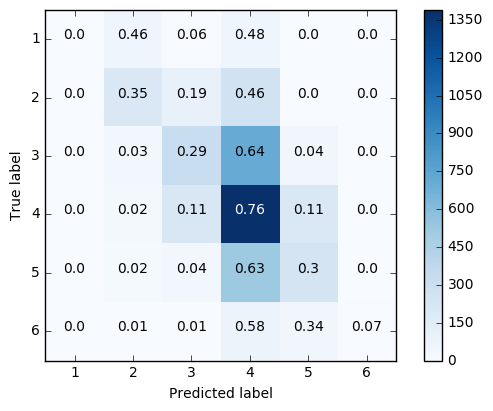
\includegraphics[width=.95\linewidth]{img/celeb_lin_cm_retweets}
  \caption{Celebrity data set}
  \label{fig:retw_distr_sub1}
\end{subfigure}%
\begin{subfigure}{.5\textwidth}
  \centering
  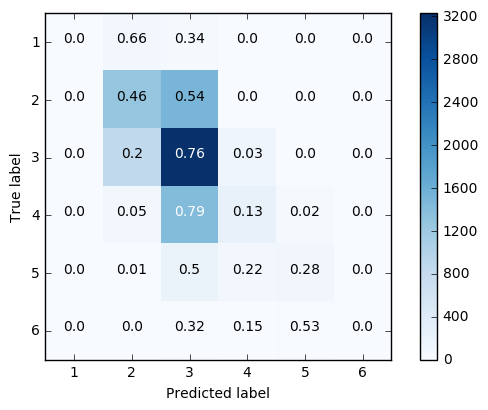
\includegraphics[width=.95\linewidth]{img/polit_lin_cm_retweets}
  \caption{Politician data set}
  \label{fig:retw_distr_sub2}
\end{subfigure}
\begin{subfigure}{.5\textwidth}
  \centering
  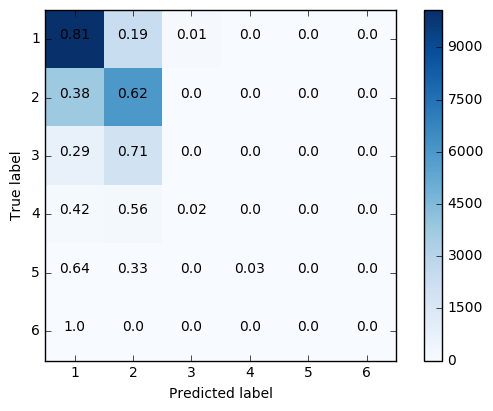
\includegraphics[width=.95\linewidth]{img/corp_lin_cm_retweets}
  \caption{Company data set}
  \label{fig:retw_distr_sub3}
\end{subfigure}%
\caption{Confusion matrices for linear retweet classification models}
\label{fig:lin_cm}
\end{figure}

More detailed observations about classification performance can be derived from
looking at confusion matrices (see Fig.~\ref{fig:lin_cm}).
These illustrations contrast predicted and actual classes for all three data sets.
For example, entry $c_{ij}$ denotes which percentage of examples in class $i$
were placed in class $j$ by the classifier.
Hence, high percentages on the main diagonal are desirable for a solid classifier.
In addition to these normalized values, color maps illustrate the absolute
number of predictions for a particular class combination.
It can be stated that all models are biased towards larger classes, i.e.,
most examples are simply placed in these classes.
For celebrities, the most common class for celebrity tweets is 4 (100-999 retweets), while classes
3 (10-99 retweets) and 0 (zero retweets) are most frequently occurring for politician and company data
(see ch.~\ref{sec:engagement_stats}).
Accuracy for predicting these popular classes is higher than 75\% on all three data sets.
However, too many examples from other classes are misclassified here, as can be
seen when looking at respective class columns.
Such model behavior results in poor predictive performance for less common classes.
Confusion matrices for favorite prediction yield similar results and are
omitted for the sake of brevity here (see Appendix).

Analyzing above results points to an intuitive interpretation of model behavior.
All models are obviously biased towards the more common classes in a data set.
Since the company data possesses the most class imbalance (nearly 90\% of examples
stem from classes 0 and 1), linear models tend to perform better here.
Contrary, model performance decreases for wider and less imbalanced class distributions.
Two possible reasons for this kind of model bias can be derived.
Firstly, linear models have limited representational capability, i.e., a small
number of trainable parameters.
Secondly, structured input features could not be sufficient to learn acceptable
class boundaries.
For example, the actual tweet content is mostly ignored when using these simple
features.
The following sections will aim to overcome these liabilities by replacing
linear models with deep neural networks.
Adding more layers to the model architecture results in more trainable parameters
for representing inputs, which in turn should improve
model performance.
Results from training deep feedforward models on structured input data are
described in the following section (ch.~\ref{sec:deep1}).
Moreover, modeling tweet content using more sophisticated layer architectures
should enable deep neural networks to learn more meaningful features.
These additional features derived from unstructured data should also enable
more accurate engagement predictions.
Ch.~\ref{sec:deep_combined} explores possibilities for building these kinds
of more complex models.


\subsection{Deep Models on Structured Data}
\label{sec:deep1}

Linear models directly map from inputs to predictions.
Assuming the inputs stay the same, the next step in neural network evolution
should be to add hidden layers.
The reasoning behind this is the increased capability of the model to learn intermediate
feature representations, which in turn should enable more accurate predictions.
This section examines application of deep feedforward networks to the problem
of engagement prediction.
Model architectures are introduced in Chapter~\ref{sub:deep1_architecture}, 
before the training process is detailled in Chapter~\ref{sub:deep1_training}.
Finally, results and accompanying analysis are presented in Chapter~\ref{sub:deep1_performance}.

\subsubsection{Model architecture}
\label{sub:deep1_architecture}

Model architecture for the deep feedforward networks is similar to linear models
in that model inputs and outputs are the same.
The main difference is the addition of hidden layers inbetween inputs and outputs.
Fully-connected feedforward layers (see ch.~\ref{sub:dl_concepts}) are chosen,
because they constitute the sole reasonably applicable layer architecture.
More complex layer architectures like recurrent or convolutional layers require
temporal or local relations between input features.
Examples for such relations would be images (local relations between pixels)
or time-series data (obvious temporal relation).
The main question that arises is how many hidden layers should be inserted.
Additionally, the number of neurons in hidden layers has to be determined.
No strict rules exist to answer this question, but heuristics have been developed
by long-time deep learning practicioners~\footnote{\url{http://www.heatonresearch.com/2017/06/01/hidden-layers.html}}.
In any case, experimentation is required to find a suitable architecture for a distinct problem setting.
Thus, several architectures were tested for model selection in this work.
Obvious evaluation criteria are model performance on training and validation data,
as well as total training time.

\begin{table}
\begin{tabular}{llrr}
\toprule
Hidden layers & Hidden units & Classification loss & Regression loss \\
\midrule
2 & 16 & 0.8203 & 2,593.2 \\
2 & 32 & 0.7502 & 2,520.2 \\
2 & 64 & 0.7346 & 2,509.9 \\
3 & 16 & 0.7888 & 2,529.9 \\
3 & 32 & 0.7430 & 2,557.3 \\
3 & 64 & 0.7160 & 2,465.1 \\
4 & 16 & 0.7792 & 2,588.5 \\
4 & 32 & 0.7261 & 2,477.5 \\
4 & 64 & \textbf{0.7088} & 2,435.8 \\
5 & 64 & 0.7128 & \textbf{2,386.1} \\
6 & 64 & 0.7016 & 2,410.1 \\
\bottomrule
\end{tabular}
\caption{Summary of model selection results}
\label{tab:dm1_selection_results}
\end{table}

Experimentation for classification and regression models was conducted on the
celebrity data set, because it contains the smallest number of training examples
and is thus most prone to overfitting.
In order to preserve comparability, the same settings were used for each architecture.
Models were trained for 50 (classification) respectively 100 (regression) epochs
on identical training examples.
Tested variants included two to six hidden layers with the same number of hidden
units in each layer, namely 16, 32 and 64 neurons.
Some architectures for very deep networks (five or six hidden layers) were omitted
when it became obvious that layers with 64 neurons showed the most promising
performance.
Table~\ref{tab:dm1_selection_results} summarizes results for the experiments.
As expected, increases in both number of hidden layers and units improve
performance.
However, adding units yields generally leads to higher performance increases than
simply adding layers.
In addition, adding more hidden layers increases total training time more than
adding units.
Including more than four hidden layers only leads to minor performance improvement for
the classification setting.
Also, a more unstable training process was observed, sometimes resulting in overfitting.
Hence, the configuration consisting of four layers with 64 neurons each was
chosen for models in this thesis.
The regression setting proved to be a bit more robust regarding the number of
hidden layers, so that an additional layer could be inserted here.

\begin{figure}[h]
\begin{subfigure}{.4\textwidth}
  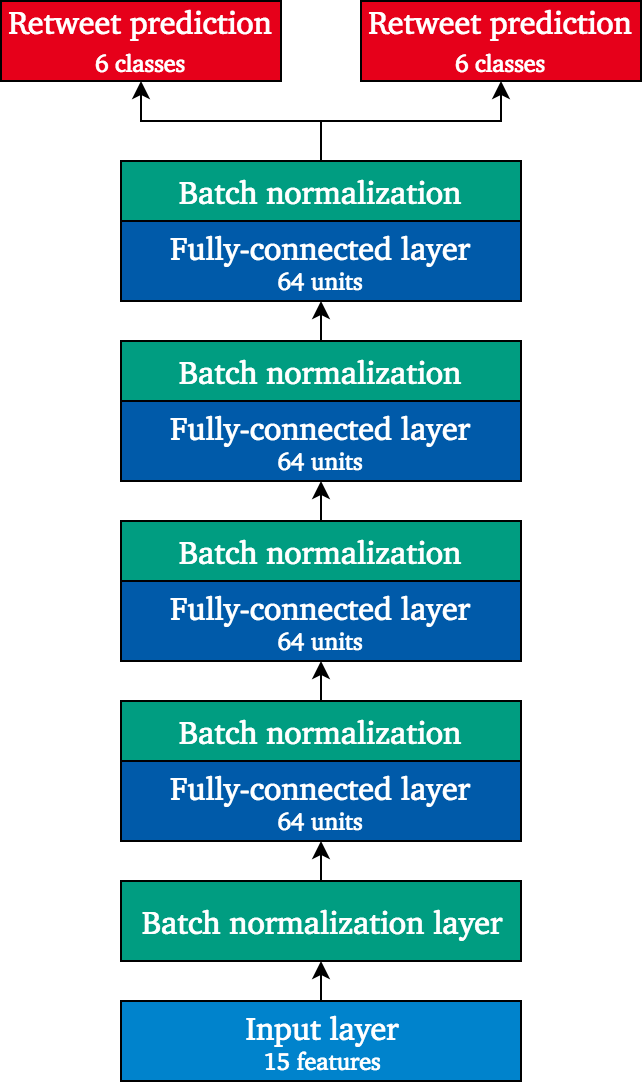
\includegraphics[width=.95\linewidth]{img/deep_1_class_architecture}
  \caption{Classification model}
  \label{fig:deep1_architecture_1}
\end{subfigure}%
\begin{subfigure}{.4\textwidth}
  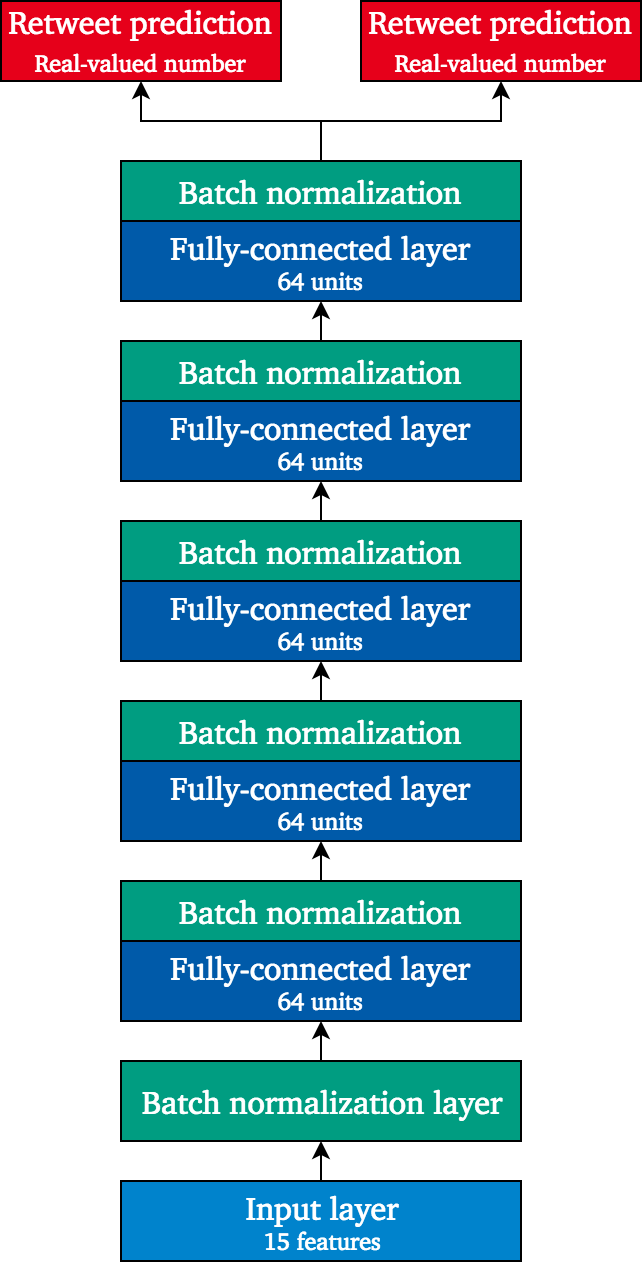
\includegraphics[width=.95\linewidth]{img/deep_1_regr_architecture}
  \caption{Regression model}
  \label{fig:deep1_architecture_2}
\end{subfigure}
\caption{Architecture of deep feedforward network}
\label{fig:deep1_architecture}
\end{figure}

Fig.~\ref{fig:deep1_architecture} shows the final neural network architectures
for this section.
Input features and output types (including classes) are identical to the ones
used in linear models (see ch.~\ref{sub:lin_architecture}).
As before, inputs are normalized using batch normalization, which is also applied
after each fully-connected layer.
Citing Chapter~\ref{sub:dl_developments}, batch normalization speeds up the
training process by decreasing the range of weight values without sacrificing
model performance.
Moreover, it helps to avoid overfitting, which is more prone to occur in models
containing many learnable parameters.

\subsubsection{Training process}
\label{sub:deep1_training}

\outline{Setting is mostly unchanged: same training/validation split, optimizer
and cost functions}
\outline{Only change: regression model trained for only 100 iterations since they
converge faster}

\subsubsection{Model performance}
\label{sub:deep1_performance}

\begin{table}
  \begin{tabular}{lrrrrrrr}
    \toprule
    & \multicolumn{4}{l}{Classification} & \multicolumn{3}{l}{Regression} \\
    \midrule
    Data set & CCE & Acc & Ret Acc & Fav Acc & MAE & Ret MAE & Fav MAE \\
    \midrule
    Celebrities & 0.71 & 70.29\% & 66.30\% & 74.28\% & 2,345.85 & 1,165.19 & 3,526.51 \\
    Politicians & 0.81 & 64.75\% & 63.37\% & 66.12\% & 424.05 & 247.40 & 600.69 \\
    Companies & 0.72 & 70.07\% & 72.38\% & 67.76\% & 19.72 & 10.92 & 28.52 \\
    Combined & 1.03 & 55.50\% & 57.75\% & 53.25\% & 549.93 & 210.71 & 889.16 \\
    \bottomrule
  \end{tabular}
  \caption{Summary of results for deep feedforward network}
  \label{tab:deep1_results}
\end{table}

\outline{Overall performance increases (cost function lower for both tasks
across all data sets)}
\outline{Additional information: models start to overfit slightly (esp. company
classification => training loss is 0.64)}
\outline{Classification accuracy improvements between 10 and 20 \% (celebrity performance
improvements are strongest), 65 to 70\% of validation examples are classified correctly}
\outline{Improvements are slightly higher for favorite classification (except for politicians)}
\outline{Relation between RetAcc and FavAcc unchanged}
\outline{Interesting: classification works best for celebrity data (previously worst performance)}
\outline{MAE results lowered by 12 (politicians) to 33\% (celebrities)}
\outline{Improvements mostly driven by strong decreases in FavMAE (decreases
higher across the board)}
\outline{More details on classification and regression performance in the following}

\begin{figure}[h]
\begin{subfigure}{.5\textwidth}
  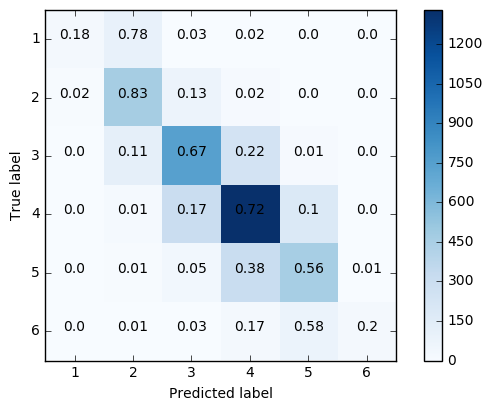
\includegraphics[width=.95\linewidth]{img/celeb_d1_cm_retweets}
  \caption{Celebrity data set}
  \label{fig:retw_distr_sub1}
\end{subfigure}%
\begin{subfigure}{.5\textwidth}
  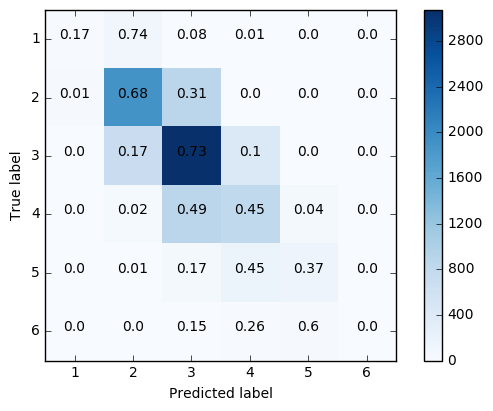
\includegraphics[width=.95\linewidth]{img/polit_d1_cm_retweets}
  \caption{Politician data set}
  \label{fig:retw_distr_sub2}
\end{subfigure}
\begin{subfigure}{.5\textwidth}
  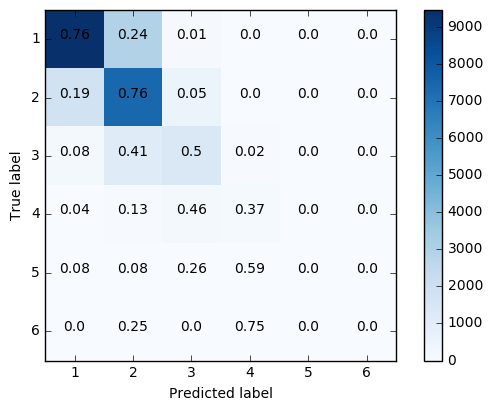
\includegraphics[width=.95\linewidth]{img/corp_d1_cm_retweets}
  \caption{Company data set}
  \label{fig:retw_distr_sub3}
\end{subfigure}%
\begin{subfigure}{.5\textwidth}
  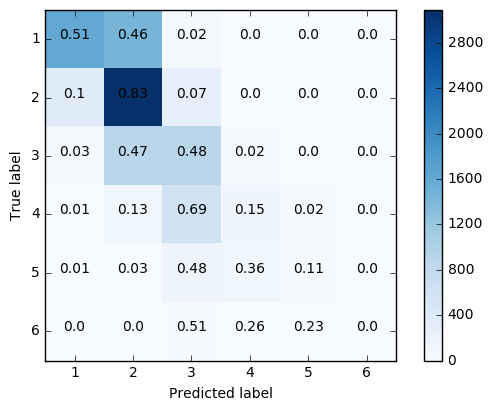
\includegraphics[width=.95\linewidth]{img/comb_d1_cm_retweets}
  \caption{Combined data set}
  \label{fig:retw_distr_sub4}
\end{subfigure}%
\caption{Confusion matrices for deep feedforward classification models}
\label{fig:d1_cm}
\end{figure}

\outline{More correctly classified examples (see main diagonal)}
\outline{Celebrities: Classes around median are predicted more accurately than border classes}
\outline{Celebrities: Not biased towards biggest class, misclassifications are `better'}
\outline{Sames is true for politicians}
\outline{Companies: model is good at predicting first two classes}
\outline{Companies: better (but not good) performance on classes 3 and 4}
\outline{Companies: classes 5 and 6 are still never predicted}

\begin{table}
  \begin{tabular}{lrrrrrrr}
    \toprule
    & \multicolumn{7}{c}{Actual retweets} \\
    \midrule
    Data set & 0 & 1-10 & 10-100 & 100-1k & 1-10k & 10-100k & >100k \\
    \midrule
    Celebrities & - & 51.9 & 161.4 & 701.3 & 3,884.9 & 21,557.9 & - \\
    Politicians & 46.0 & 109.7 & 184.5 & 781.0 & 3,973.1 & - & - \\
    Companies & 1.5 & 5.9 & 49.5 & 605.7 & - & - & - \\
    Combined & 0.4 & 5.2 & 32.0 & 233.6 & 2,088.3 & 21,919.0 & 86,217.9 \\
    \bottomrule
    \toprule
    & \multicolumn{7}{c}{Actual favorites} \\
    \midrule
    Data set & 0 & 1-10 & 10-100 & 100-1k & 1-10k & 10-100k & >100k \\
    \midrule
    Celebrities & - & 7.4 & 268.5 & 638.1 & 3,139.2 & 19,212.0 & 45,031.3 \\
    Politicians & 92.6 & 130.4 & 234.1 & 864.5 & 3,528.9 & 12,167.6 & - \\
    Companies & 6.5 & 6.6 & 39.7 & 743.1 & 1,314.0 & - & - \\
    Combined & 0.4 & 4.4 & 32.1 & 355.8 & 3,279.5 & 26,871.1 & 169,920.5 \\
    \bottomrule
  \end{tabular}
  \caption{Mean absolute errors for specific ranges of actual engagement}
  \label{tab:d1_regression_eval}
\end{table}

\outline{Using MAE requires mean calculation => need for more detailed performance
evaluation}
\outline{Errors need to be considered in relation to magnitude of actual counts}
\outline{Table shows MAE for specific ranges of actual engagement counts}
\outline{Dash denotes absence of validation data for this range}
\outline{Observation: MAE increases with rising engagement counts}
\outline{Order of magnitudes vary drastically (can be expected)}



\section{Deep Models on Enriched Data}
\label{sec:deep_combined}

\subsection{Text preprocessing}
\label{sub:text_preprocess}

\subsection{Model architecture}
\label{sub:model_architecture}

\subsection{Model performance}
\label{sub:comb_performance}

\section{Summary}
\label{sec:res_summary}
